% !TeX root = ../main_ustc.tex
\chapter{控制理论基础}
\label{chap:preliminaries}

人机协同柔性接触操作需要同时解释机器人运动、环境形变、接触力反馈和多目标权衡。自由空间轨迹跟踪主要关注末端位姿误差，柔性接触任务中的末端位移还会通过接触几何转化为材料变形，材料变形又以接触力形式作用于机器人和操作者。围绕这一物理链条，本章建立任务空间模型、柔性接触模型、力位协同方法，并在多目标优化意义下介绍合作博弈理论和线性二次型最优控制基础。稳定性分析所需的二次型值函数、黎卡提方程和扰动有界处理融入相关模型与控制理论中，使本章内容能够作为全文控制问题建模和分析的理论基础。

\section{任务空间建模基础}
\label{sec:ch2_robotics}

机器人运动学描述关节变量与末端位姿之间的几何关系，动力学描述关节力矩、惯性、重力、外部作用力与运动之间的关系。相关基础在机器人学教材、机器人学手册和操作空间控制文献中已有系统总结\cite{murray1994mathematical,siciliano2016handbook,khatib1987operational}。对于柔性接触操作任务，运动学用于描述末端接触点、工具轴线和几何边界，动力学用于描述机器人控制输入、环境接触力和末端运动之间的关系。

\begin{figure}[H]
  \centering
  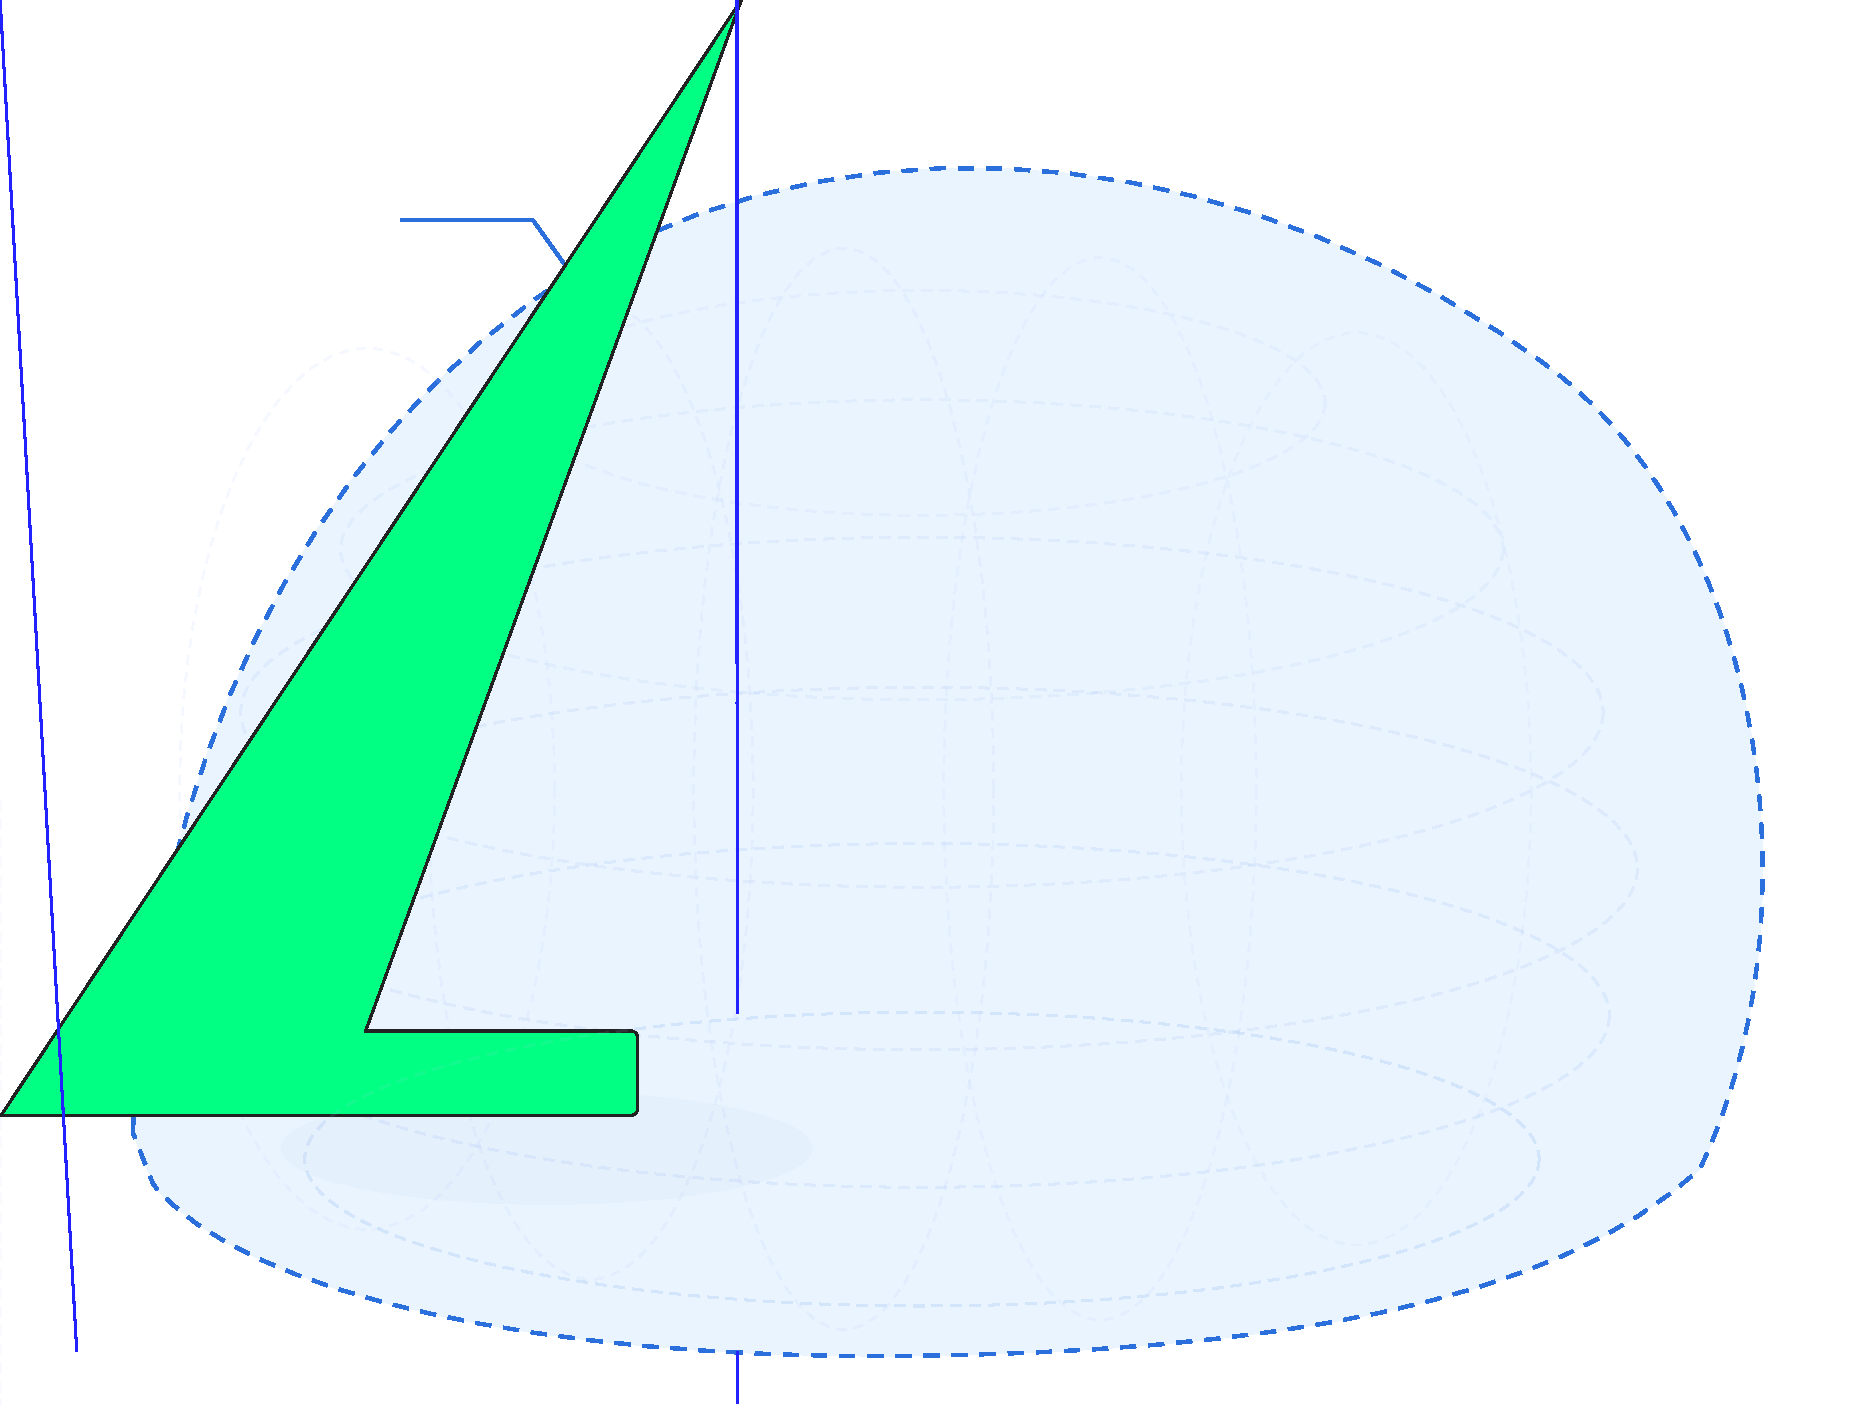
\includegraphics[width=0.88\textwidth]{figures/ch2/机械臂任务空间建模_右手系_投影修正版.pdf}
  \caption{机械臂任务空间建模示意图}
  \label{fig:ch2_task_space_mapping}
\end{figure}

图\ref{fig:ch2_task_space_mapping} 给出了机械臂任务空间建模的基本对象。基座坐标系 $\{B\}$ 采用右手系描述机器人安装基准和全局运动方向，末端坐标系 $\{E\}$ 描述工具或末端执行器的局部位姿；任务空间中的位置向量 $p=[x,y,z]^\mathrm{T}$ 表示末端在基座坐标系下的空间坐标，期望位置 $p_d=[x_d,y_d,z_d]^\mathrm{T}$ 则给出了控制任务希望末端到达或跟踪的目标。图中投影关系说明，三维末端运动可以分解到不同坐标方向进行误差度量和控制分析。由此可见，任务空间建模的核心是把关节变量映射为末端位置、姿态和速度，并进一步建立目标轨迹、末端误差和外部作用力之间的关系。

设机械臂具有 $n_q$ 个自由度，关节位置、速度和加速度分别记为 $q,\dot q,\ddot q\in\R^{n_q}$。任务空间变量记为 $x\in\R^m$，其中 $m$ 表示任务空间维数。若仅考虑末端平移运动，通常取 $m=3$；若同时考虑位置和姿态，可取 $m=6$。机械臂正运动学映射可表示为
\begin{equation}
  x=\Phi(q),
  \label{eq:ch2_forward_kinematics}
\end{equation}
其中 $\Phi(\cdot)$ 为由关节空间到任务空间的非线性映射。对\eqref{eq:ch2_forward_kinematics}求导得到速度关系
\begin{equation}
  \dot x=J(q)\dot q,
  \label{eq:ch2_jacobian_velocity}
\end{equation}
其中 $J(q)\in\R^{m\times n_q}$ 为机械臂雅可比矩阵。进一步求导得到加速度关系
\begin{equation}
  \ddot x=J(q)\ddot q+\dot J(q,\dot q)\dot q .
  \label{eq:ch2_jacobian_acceleration}
\end{equation}
式中 $\dot J(q,\dot q)\dot q$ 表示雅可比矩阵随关节运动变化而产生的速度相关项。上述关系说明，末端速度和加速度不仅由关节速度和关节加速度决定，还与当前构型有关；当机械臂靠近奇异位形时，较小的末端运动可能对应较大的关节速度或力矩需求。

\begin{definition}[任务空间误差变量]
\label{def:ch2_task_error}
任务空间期望轨迹记为 $x_d(t)$，其速度和加速度分别为 $\dot x_d(t)$ 和 $\ddot x_d(t)$。任务空间位置误差和速度误差定义为
\begin{equation}
  e_x(t)=x(t)-x_d(t),\qquad e_v(t)=\dot x(t)-\dot x_d(t).
  \label{eq:ch2_basic_errors}
\end{equation}
其中 $e_x$ 表示实际末端位置相对于期望位置的偏差，$e_v$ 表示实际末端速度相对于期望速度的偏差。二者是任务空间反馈控制、阻抗控制和轨迹跟踪性能评价中的基本误差量。
\end{definition}

机械臂关节空间动力学通常写为
\begin{equation}
  M_q(q)\ddot q+C_q(q,\dot q)\dot q+G_q(q)=\tau+\tau_{\mathrm{ext}},
  \label{eq:ch2_joint_dynamics}
\end{equation}
其中 $M_q(q)\in\R^{n_q\times n_q}$ 为关节空间惯性矩阵，$C_q(q,\dot q)\dot q$ 为科氏力和离心力项，$G_q(q)$ 为重力项，$\tau\in\R^{n_q}$ 为关节驱动力矩，$\tau_{\mathrm{ext}}\in\R^{n_q}$ 为外部作用力映射到关节空间后的广义力矩。若任务空间广义力或六维广义力记为 $w$，则由虚功原理得到
\begin{equation}
  \tau_{\mathrm{ext}}=J^T(q)w .
  \label{eq:ch2_jacobian_transpose}
\end{equation}
该关系表明，环境接触力、操作者交互力或工具受力会通过雅可比转置映射到关节空间。接触任务中的力安全问题会同时体现在末端、关节驱动、传感器量程和控制输入饱和等环节。

\begin{assumption}[机械臂模型的正则性]
\label{ass:ch2_robot_regular}
在本文考虑的工作空间内，惯性矩阵 $M_q(q)$ 一致正定；矩阵 $M_q(q)$、$C_q(q,\dot q)$、$G_q(q)$ 以及雅可比矩阵 $J(q)$ 关于其自变量连续。机械臂运动范围避开运动学奇异区域，使得所需任务空间映射在局部有定义。
\end{assumption}

\begin{remark}
\cref{ass:ch2_robot_regular} 是机械臂控制分析中的常用基本条件。该条件关注机器人在实验工作区间内的运动学和动力学正则性，动力学参数精度只需满足局部建模和反馈控制分析的基本需求，使任务空间建模和局部反馈控制具有物理意义。
\end{remark}

在机器人操作任务中，控制目标通常直接给定在任务空间。由关节空间动力学和雅可比映射可得到任务空间动力学的一般形式
\begin{equation}
  M_x(q)\ddot x+C_x(q,\dot q)\dot x+G_x(q)=u_x+f_{\mathrm{ext}},
  \label{eq:ch2_task_dynamics}
\end{equation}
其中 $M_x(q)$ 为任务空间惯性矩阵，$C_x(q,\dot q)\dot x$ 为任务空间速度相关项，$G_x(q)$ 为任务空间重力项，$u_x$ 为任务空间控制输入，$f_{\mathrm{ext}}$ 为环境或人机交互产生的外部作用力。对于已经具备高带宽内环、重力补偿或笛卡尔伺服接口的机器人，也可在工作点附近将任务空间误差模型抽象为
\begin{equation}
  \dot x_s=A_sx_s+B_su,
  \label{eq:ch2_general_state_space}
\end{equation}
其中 $x_s$ 为一般状态向量，$u$ 为控制输入，$A_s$ 和 $B_s$ 为相应系统矩阵。若存在二次型函数 $V=x_s^TPx_s$，且在局部区域内满足
\begin{equation}
  \underline p\norm{x_s}^2\le V\le \bar p\norm{x_s}^2,\qquad
  \dot V\le -c\norm{x_s}^2,
  \label{eq:ch2_lyap_embedded}
\end{equation}
其中 $\underline p$、$\bar p$ 和 $c$ 为正常数，则可由李雅普诺夫方法得到闭环状态的指数衰减界\cite{khalil2002nonlinear}。该结论在控制理论中用于说明二次型能量函数随闭环演化下降，其物理含义是位置、速度或力误差的综合能量被反馈控制持续耗散。

\section{柔性接触建模基础}
\label{sec:ch2_contact_modeling}

柔性接触建模的核心在于描述末端运动、环境变形和接触力之间的关系。与刚性接触不同，柔性材料、软组织、橡胶件或复合材料表面在受力后会产生可观测形变，接触区域、接触法向和等效刚度也可能随时间变化。接触力学和接触动力学研究通常从局部几何、材料等效刚度、阻尼耗散和接触状态切换等方面描述这一过程\cite{johnson1985contact,gilardi2002survey}。充分描述这种耦合关系，有助于避免控制器把位置误差直接转化为过大的法向压入，也有助于在力控过程中保留必要的切向运动。

图\ref{fig:ch2_kelvin_voigt_contact} 展示了局部柔性接触的物理示意和等效力学关系。末端与柔性环境接触时，压入量 $\delta$ 和压入速度 $\dot{\delta}$ 共同决定局部接触响应；弹簧项 $K_e\delta$ 描述材料变形产生的回复力，阻尼项 $B_e\dot{\delta}$ 描述接触过程中的耗散作用。该图强调本文采用的是工作点附近的局部等效模型，其作用在于把柔性环境形变转化为可进入控制器设计与实验分析的接触力近似。

\begin{figure}[H]
  \centering
  \includegraphics[width=0.82\textwidth]{figures/ch2/kelvin_voigt_flexible_contact_vector.pdf}
  \caption{柔性环境接触建模的开尔文--沃伊特模型}
  \label{fig:ch2_kelvin_voigt_contact}
\end{figure}

在局部接触范围内，柔性环境可由黏弹性本构关系和局部接触力学近似描述\cite{christensen1982viscoelasticity,johnson1985contact}。机器人接触控制中常将接触点附近的环境等效为弹簧--阻尼并联模型，接触阻抗估计和 Hunt--Crossley 动态接触模型辨识研究也表明，压入量、压入速度、等效刚度和等效阻尼是描述局部动态接触的基本变量\cite{hunt1975coefficient,diolaiti2005contact,haddadi2012huntcrossley}。在工作点附近取线性近似时，开尔文--沃伊特模型可写为
\begin{equation}
  f_e=K_e\delta+B_e\dot\delta+\Delta_f,
  \label{eq:ch2_kelvin_voigt}
\end{equation}
其中 $f_e$ 为环境接触力，$K_e\succeq0$ 为等效刚度矩阵，$B_e\succeq0$ 为等效阻尼矩阵，$\delta$ 为压入量，$\dot\delta$ 为压入速度，$\Delta_f$ 表示未建模非线性、参数变化和测量误差引起的接触模型误差。该模型的物理含义较为直观：同样的压入深度在不同刚度区域会产生不同的接触力，同样的末端速度在不同阻尼条件下会产生不同的耗散力。

给定期望接触力 $f_d$，力误差定义为
\begin{equation}
  e_f=f_e-f_d .
  \label{eq:ch2_force_error}
\end{equation}
其中 $e_f$ 反映实际接触力偏离期望接触力的程度。为了减小静态误差并避免普通积分项在长时间接触中无界增长，可采用泄漏积分状态
\begin{equation}
  \dot\sigma_f=e_f-\lambda_f\sigma_f,
  \label{eq:ch2_leakage_integral}
\end{equation}
其中 $\sigma_f$ 为力误差泄漏积分状态，$\lambda_f>0$ 为泄漏系数。泄漏项使积分状态在力误差消失后逐渐衰减，能够降低传感器偏置、材料蠕变和慢变模型误差对控制输入的持续影响。这一处理与控制工程中通过泄漏项或抗积分饱和机制限制积分状态长期累积的思想一致\cite{astrom2006advanced,khalil2002nonlinear}。

\begin{assumption}[接触模型的局部有界性]
\label{ass:ch2_contact_bounded}
在本文考虑的接触任务区间内，环境等效刚度和阻尼有界，接触模型误差 $\Delta_f$ 有界。若将参考轨迹变化、接触面运动、参数失配和传感噪声统一为残差项，则该残差项在局部紧集内有界。
\end{assumption}

\begin{remark}
\cref{ass:ch2_contact_bounded} 允许柔性环境存在非线性和未知接触参数，其核心限定是分析对象处于有限工作区间，且模型残差保持有界。机器人接触阻抗估计和接触模型辨识研究通常也在有限工作区间内处理等效刚度、阻尼和模型误差的估计问题\cite{diolaiti2005contact,haddadi2012huntcrossley}。对于实际机器人接触任务，这一条件通常通过工作空间限制、力阈值保护、速度限幅和传感器滤波共同保证。
\end{remark}

在固定通道、夹具、导向孔或长工具操作中，柔性接触还会受到几何边界影响。一般约束可写为
\begin{equation}
  h(x,q,t)=0,
  \label{eq:ch2_general_constraint}
\end{equation}
其中 $h(\cdot)$ 为约束函数，$x$ 为任务空间变量，$q$ 为关节变量。若约束表现为固定点与工具轴线之间的距离约束，可定义
\begin{equation}
  e_c(t)=\dist(p_c,\ell(t)),
  \label{eq:ch2_constraint_error}
\end{equation}
其中 $p_c\in\R^3$ 为固定约束点，$\ell(t)$ 为工具轴线，$\dist(\cdot)$ 表示点到直线的欧氏距离。当 $e_c(t)$ 较小时，工具轴线在允许误差范围内经过固定点；当该误差增大时，工具可能对通道、夹具或组织入口产生不期望的横向作用。微创手术中的远心运动约束（remote center of motion, RCM）就是固定点--轴线几何约束的典型形式，其中固定点对应穿刺孔或套管入口，工具轴线需要在操作过程中尽量经过该固定点\cite{aghakhani2013task,kastritsi2021rcmcontroller,zhang2024rcmreview}。工业导向孔、深腔入口和夹具中心虽然应用背景不同，也可用相同几何关系描述。

\begin{definition}[固定点--轴线几何约束]
\label{def:ch2_point_axis_constraint}
若机器人末端工具轴线 $\ell(t)$ 需要经过固定点 $p_c$，则称该操作满足固定点--轴线几何约束。该定义是对远心运动约束中器械轴线经过固定远心点这一几何要求的抽象化表述\cite{aghakhani2013task,kastritsi2021rcmcontroller,kastritsi2022passiveadmittance}。约束误差由\eqref{eq:ch2_constraint_error}给出。当 $e_c(t)=0$ 时，工具轴线严格通过固定点；当 $e_c(t)$ 有界且足够小时，几何约束在允许误差范围内得到保持。
\end{definition}

接触模型误差通常可以并入状态方程残差。若残差项 $d(x_s,t)$ 满足
\begin{equation}
  \norm{d(x_s,t)}\le \bar d_0+\bar d_1\norm{x_s},
  \label{eq:ch2_disturbance_bound}
\end{equation}
其中 $\bar d_0$ 和 $\bar d_1$ 为非负常数。在鲁棒非线性控制分析中，类似有界残差常用于描述参数摄动、未建模动态和外部扰动对闭环系统的影响\cite{khalil2002nonlinear}。进一步利用杨氏不等式
\begin{equation}
  2a^Tb\le \varepsilon\norm{a}^2+\frac{1}{\varepsilon}\norm{b}^2,\qquad \varepsilon>0
  \label{eq:ch2_young}
\end{equation}
将值函数导数中的扰动交叉项转化为状态二次项和残差界。该处理说明模型误差的影响会体现为闭环有界邻域的扩大。柔性接触控制的保守性很大程度上来自这里：模型精度越低，控制器越需要保留更大的力安全裕度和更慢的参数变化。

\section{力位协同控制方法}
\label{sec:ch2_impedance_force_position}

机器人与环境接触或与操作者交互时，单纯的位置控制容易产生较大的交互力。阻抗控制通过指定运动误差与外部力之间的动态关系，使机器人表现出期望的柔顺特性，是机器人接触控制和物理人机交互中的基础方法之一\cite{hogan1985impedance,haddadin2016physical,calanca2016compliant,ficuciello2015variable}。

\begin{figure}[H]
  \centering
  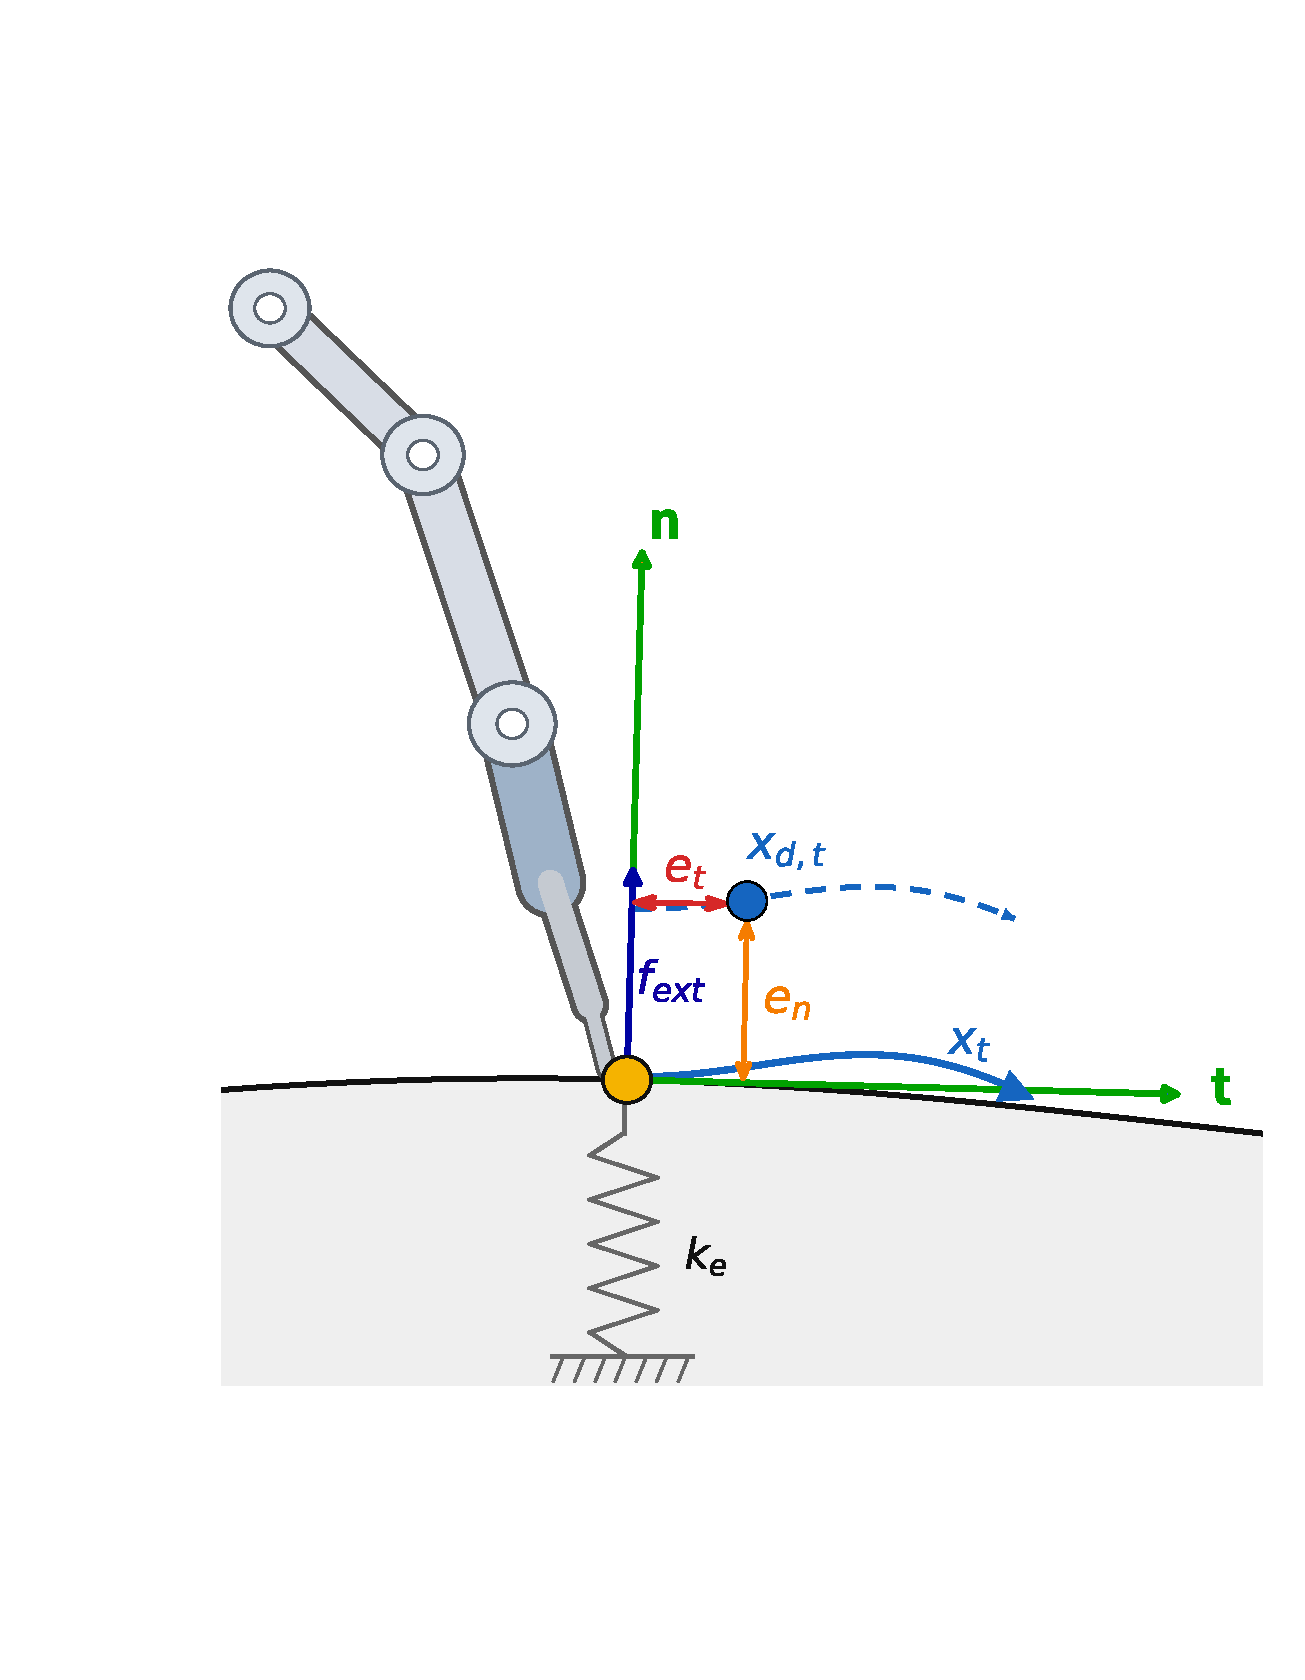
\includegraphics[width=0.72\textwidth]{figures/ch2/接触任务几何与误差分解_矢量.pdf}
  \caption{接触任务几何误差分解示意图}
  \label{fig:ch2_force_position_coordination}
\end{figure}

如图\ref{fig:ch2_force_position_coordination} 所示，接触点处的局部坐标可分解为切向方向 $t$ 和法向方向 $n$。切向位置 $x_t$ 与期望切向位置 $x_{d,t}$ 之间形成切向误差 $e_t$，该误差主要影响扫描覆盖、加工路径和任务完成质量；法向误差 $e_n$ 则对应末端相对柔性表面的压入或脱离趋势，并通过环境等效刚度 $k_e$ 反映到外部接触力 $f_{\mathrm{ext}}$ 中。由此可见，接触任务中的位置目标和力目标具有明确方向属性，力位协同控制需要在切向轨迹精度、法向接触稳定性和力安全边界之间分配控制优先级。

在任务空间中，典型阻抗模型可写为
\begin{equation}
  M_d(\ddot x-\ddot x_d)+D_d(\dot x-\dot x_d)+K_d(x-x_d)=f_{\mathrm{ext}},
  \label{eq:ch2_impedance}
\end{equation}
其中 $M_d\succ0$、$D_d\succ0$ 和 $K_d\succeq0$ 分别为期望惯性、阻尼和刚度矩阵，$f_{\mathrm{ext}}$ 为外部作用力。刚度矩阵主要决定位置偏差对应的回复作用，阻尼矩阵主要决定速度偏差和振荡衰减，惯性矩阵影响瞬态响应。较大的刚度通常有利于减小轨迹误差，但在柔性环境刚度较高时可能放大法向接触力；较小的刚度有利于柔顺交互，却可能造成轨迹漂移和任务覆盖不足。

\begin{definition}[任务空间阻抗]
\label{def:ch2_impedance}
若机器人末端在外力作用下满足形如\eqref{eq:ch2_impedance}的力--运动动态关系，则称该机器人在任务空间呈现由 $M_d$、$D_d$ 和 $K_d$ 描述的机械阻抗。阻抗矩阵决定了机器人在交互过程中的柔顺性、响应速度和接触稳定性。
\end{definition}

阻抗控制物理含义清楚，参数调节直观，在环境模型精度有限时仍能提供柔顺交互。其适用边界在于：阻抗参数一旦固定，位置精度和接触力安全之间的折中关系也随之固化。当环境刚度、接触法向或任务阶段发生变化时，固定阻抗同时保持较小轨迹误差和较小力误差的能力会受到影响。自适应阻抗和变阻抗控制通过在线调节刚度、阻尼或惯性来增强适应性，但参数变化仍需满足稳定性和安全性要求\cite{calanca2016compliant,ficuciello2015variable}。

力位混合控制从另一个角度处理接触任务。该方法通过选择矩阵区分自由运动方向和受约束方向：在自由方向跟踪位置或速度，在约束方向调节接触力\cite{mason1981compliance,raibert1981hybrid,khatib1987operational}。设 $S_p$ 和 $S_f$ 分别为位置控制方向和力控制方向的选择矩阵，理想正交分解下可满足
\begin{equation}
  S_p+S_f=I,\qquad S_pS_f=0 .
  \label{eq:ch2_selection_matrices}
\end{equation}
相应目标可写为
\begin{equation}
  S_pe_x\to0,\qquad S_fe_f\to0 ,
  \label{eq:ch2_hybrid_objective}
\end{equation}
其中 $S_pe_x$ 表示自由方向上的位置误差，$S_fe_f$ 表示约束方向上的接触力误差。对于刚性环境和明确约束方向，该思想非常有效；对于柔性环境，受力方向、接触区域和等效刚度可能随末端运动变化，单纯依赖固定方向分解会遇到困难。尤其在人机协同任务中，操作者输入可能同时包含切向修正和法向压入，控制器需要判断哪些运动应被视为任务修正，哪些运动会引起接触风险。

力位协同控制关注的是同一接触任务中的两类目标：位置目标要求机器人沿期望轨迹运动，力目标要求接触力保持在期望值或安全范围附近。二者具有耦合关系，共同决定任务质量。以表面扫描为例，切向位置误差影响覆盖区域，法向力误差影响接触可靠性和材料安全；以抛光或打磨为例，轨迹决定加工均匀性，接触力影响材料去除率和工具寿命。因此，力位协同控制需要同时建模运动误差、接触力误差和控制输入，并在任务状态变化时调整二者的相对重要性。一般地，可将该类问题写成受约束多目标最优控制形式
\begin{equation}
  \min_{u(\cdot)}\int_0^T
  \left(e_x^TQ_xe_x+e_f^TQ_fe_f+u^TRu\right)\dd t ,
  \label{eq:ch2_force_position_cost}
\end{equation}
并满足
\begin{equation}
  \dot x_s=f_s(x_s,u,t),\qquad
  f_{\min}\le f_e\le f_{\max},\qquad
  u\in\mathcal U .
  \label{eq:ch2_force_position_constraints}
\end{equation}
其中 $Q_x\succeq0$、$Q_f\succeq0$ 和 $R\succ0$ 分别为位置误差、力误差和控制输入权重，$f_{\min}$ 与 $f_{\max}$ 为接触力安全边界，$\mathcal U$ 为输入可行集。该表达把轨迹精度、接触安全和控制能量放在统一框架内，也说明力位控制的关键在于在物理约束下分配不同目标的重要性。

当状态约束、输入约束和力安全边界需要显式处理时，模型预测控制和控制屏障函数二次规划提供了常用工具\cite{rawlings2017mpc,ames2017cbf,ames2019cbf}。模型预测控制能够在有限预测时域内处理多目标优化和约束，但在线计算负担与模型精度要求较高；控制屏障函数二次规划适合将安全约束写成实时可求解的二次规划，但通常需要明确的约束函数和相对阶条件。阻抗控制、力位混合控制、模型预测控制和安全二次规划各有优势，也说明柔性接触力位协同本质上是一个多目标、受约束且需要实时求解的控制问题。

\section{合作博弈理论基础}
\label{sec:ch2_game_control}

博弈论研究多个参与方在相互影响条件下的决策问题。与单目标最优控制相比，博弈论更强调不同目标或参与方之间的关系结构。微分博弈进一步把这种决策关系放入动态系统中，系统状态随时间演化，参与方的控制输入共同影响状态轨迹和性能指标。动态博弈和线性二次型动态优化的系统理论可参考相关专著\cite{basar1999dynamic,engwerda2005lqdg,anderson2007optimal}。

考虑动态系统
\begin{equation}
  \dot x_s=f(x_s,u_1,u_2,\ldots,u_N,t),
  \label{eq:ch2_game_system}
\end{equation}
其中 $x_s$ 为系统状态，$u_i$ 为第 $i$ 个参与方的控制输入。第 $i$ 个参与方的性能指标可表示为
\begin{equation}
  J_i=\int_0^\infty g_i(x_s,u_1,u_2,\ldots,u_N,t)\dd t,
  \label{eq:ch2_game_cost}
\end{equation}
其中 $g_i$ 为瞬时代价。给定初始状态后，值函数用于描述某一策略类下从当前状态出发能够获得的最优累计代价，可写为
\begin{equation}
  V_i(x_s,t)=\inf_{u_i(\cdot)}
  \int_t^\infty g_i(x_s,u_i,u_{-i},\tau)\dd \tau ,
  \label{eq:ch2_value_function}
\end{equation}
其中 $u_{-i}$ 表示除第 $i$ 个参与方以外的策略组合。与值函数对应的哈密顿函数定义为
\begin{equation}
  \mathcal H_i(x_s,u_i,u_{-i},\nabla V_i,t)
  =g_i(x_s,u_i,u_{-i},t)+\nabla V_i^Tf(x_s,u_i,u_{-i},t).
  \label{eq:ch2_hamiltonian_game}
\end{equation}
在动态规划意义下，最优策略通常由哈密顿--雅可比方程或哈密顿--雅可比--贝尔曼方程刻画。根据参与方目标之间的关系，微分博弈通常可分为非合作博弈、零和博弈和合作博弈。零和博弈强调一方收益与另一方损失相抵，适合描述对抗性控制或最坏情况扰动；非合作博弈假设各参与方分别优化自己的代价函数，均衡概念通常由纳什均衡描述；合作博弈则允许参与方以整体目标或联合收益为依据协同行动。

\begin{definition}[纳什均衡]
\label{def:ch2_nash}
给定控制策略组 $(u_1^*,u_2^*,\ldots,u_N^*)$，若对任意参与方 $i$ 和任意可行替代策略 $u_i$，都有
\begin{equation}
  J_i(u_i^*,u_{-i}^*)\le J_i(u_i,u_{-i}^*),
  \label{eq:ch2_nash}
\end{equation}
则称该策略组为纳什均衡。其中 $u_{-i}^*$ 表示除第 $i$ 个参与方以外其他参与方的均衡策略。
\end{definition}

非合作博弈的核心是个体理性。每个参与方在其他参与方策略给定时保持当前策略最优，这使纳什均衡适合描述目标存在冲突、代价函数分属不同主体或需要考虑策略竞争的场景。其适用边界也较明显：均衡结果可能偏离整体性能最优，不同参与方代价函数之间的权衡关系也可能较弱。在接触操作这类工程任务中，位置精度、接触力安全和控制输入能量通常共同服务于同一任务目标，将这些指标写成合作目标更符合任务物理含义。

\begin{definition}[微分合作博弈]
\label{def:ch2_cooperative_game}
若多个目标或参与方作用于同一连续时间动态系统
\[
  \frac{\dd x_s(t)}{\dd t}
  =f\bigl(x_s(t),u_1(t),u_2(t),\ldots,u_N(t),t\bigr),
  \qquad x_s(0)=x_{s0},
\]
并且这些参与方的代价函数可以通过共同优化准则协调，例如构造联合性能指标
\[
  J_c(u_1,\ldots,u_N)=\sum_{i=1}^{N}\omega_iJ_i,
  \qquad \omega_i\ge0,\quad \sum_{i=1}^{N}\omega_i=1,
\]
则称该问题为微分合作博弈问题。其中，``微分''体现在状态 $x_s(t)$ 作为随时间演化的动态变量，由微分方程决定；各参与方的控制输入 $u_i(t)$ 通过改变状态导数 $\dd x_s/\dd t$ 共同影响未来状态轨迹和累计代价。控制律的设计目标是在该动态演化约束下得到满足整体性能折中的控制策略。
\end{definition}

合作博弈的优势在于可以把多个性能目标放在同一个优化框架下处理。对于力位协同控制，位置误差和力误差共同服务于接触任务完成质量。合作博弈通过联合代价、权重分配和帕累托有效性描述多目标折中，使控制器设计者能够明确说明某一控制律偏向位置精度、力安全还是控制能量节约。与固定阻抗参数相比，合作博弈给出了更显式的目标层解释；与一般在线优化相比，线性二次型合作博弈还可以借助黎卡提方程得到结构清楚的反馈律。

考虑两个性能指标 $J_1$ 和 $J_2$，并定义性能向量
\begin{equation}
  \mathcal J(u)=
  \begin{bmatrix}
    J_1(u) & J_2(u)
  \end{bmatrix}^T ,
  \label{eq:ch2_performance_vector}
\end{equation}
其中 $u$ 表示可行控制律或可行策略。所有可行控制律对应的性能向量构成可行性能集合
\begin{equation}
  \mathcal P=\{\mathcal J(u)\mid u\in\mathcal U\},
  \label{eq:ch2_performance_set}
\end{equation}
其中 $\mathcal U$ 为可行控制律集合。若存在 $\tilde p,p\in\mathcal P$，使得 $\tilde p_i\le p_i$ 对所有指标成立，并且至少存在一个指标满足严格不等式，则称 $\tilde p$ 支配 $p$。若性能向量 $p$ 具有如下性质：任何使某一指标严格减小的可行性能向量，都会伴随至少另一个指标增大，则称其为帕累托有效（Pareto efficient）。所有帕累托有效性能向量构成帕累托边界，可写为
\begin{equation}
  \mathcal F_P=
  \left\{p\in\mathcal P~\middle|~
  \nexists\,\tilde p\in\mathcal P:
  \tilde p_i\le p_i,~\forall i,\;
  \tilde p_j<p_j,~\exists j
  \right\}.
  \label{eq:ch2_pareto_front}
\end{equation}
该定义的物理含义是：在帕累托边界上，若希望继续减小某一类代价，通常必须付出另一类代价增大的代价。对于多目标控制问题，$J_1$ 和 $J_2$ 可表示两类需要协调的性能指标；在具体力位协同场景中，二者可根据任务需要对应到位置跟踪、接触力调节或其他评价量。

\begin{figure}[H]
  \centering
  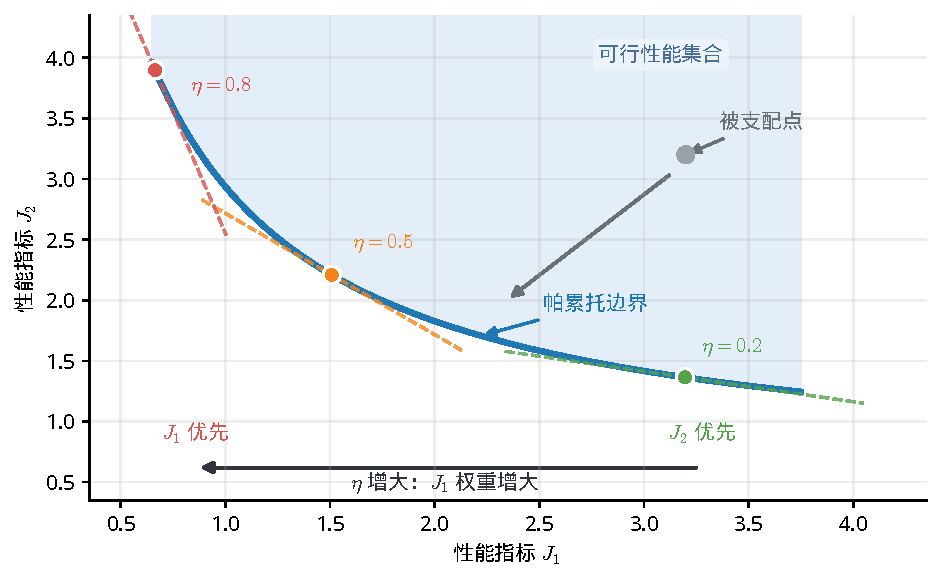
\includegraphics[width=0.86\textwidth]{figures/ch2/ch2_pareto_arbitration.pdf}
  \caption{帕累托边界与仲裁参数的几何解释}
  \label{fig:ch2_pareto_arbitration}
\end{figure}

图\ref{fig:ch2_pareto_arbitration} 直观展示了可行性能集合、帕累托边界和被支配点之间的关系。位于边界右上方的点可以同时减小两个代价，因此属于被支配解；边界上的点则代表不同控制权重下的可行工作点。在线性加权方法中，可构造
\begin{equation}
  J_\eta=\eta J_1+(1-\eta)J_2,
  \qquad \eta\in[0,1],
  \label{eq:ch2_pareto_scalarization}
\end{equation}
其中 $\eta$ 为权重参数，也可称为仲裁参数。较大的 $\eta$ 表示控制器更强调第一类性能指标，较小的 $\eta$ 表示控制器更强调第二类性能指标。对给定的 $\eta$，相应控制律可表示为
\begin{equation}
  u_\eta^*\in\argmin_{u\in\mathcal U}
  \left[\eta J_1(u)+(1-\eta)J_2(u)\right].
  \label{eq:ch2_eta_policy}
\end{equation}
不同 $\eta$ 对应帕累托边界上的不同工作点。若两个目标的可行性能集合是凸的，线性加权方法可以生成相应的帕累托有效解；当性能集合非凸时，线性加权方法可能只能得到部分帕累托边界，但它仍然具有参数含义清楚和计算结构简单的优势。

\begin{lemma}[加权代价的正定性]
\label{lem:ch2_weight_positive}
设 $Q_1\succeq0$、$Q_2\succeq0$、$R_1\succ0$、$R_2\succ0$，并令
\begin{equation}
  Q_\eta=\eta Q_1+(1-\eta)Q_2,
  \qquad
  R_\eta=\eta R_1+(1-\eta)R_2 .
\end{equation}
若 $\eta\in[0,1]$，则 $Q_\eta\succeq0$ 且 $R_\eta\succ0$。
\end{lemma}

\begin{proof}
对任意非零向量 $v$，有
\begin{equation}
  v^TR_\eta v=\eta v^TR_1v+(1-\eta)v^TR_2v .
\end{equation}
由于 $R_1\succ0$、$R_2\succ0$ 且 $\eta\in[0,1]$，上式严格大于零，因此 $R_\eta\succ0$。同理，对任意向量 $v$，$v^TQ_\eta v$ 为两个非负数的凸组合，故 $Q_\eta\succeq0$。引理得证。
\end{proof}

在线性二次型情形下，最优控制律可以由哈密顿--雅可比--贝尔曼方程推导。考虑线性系统
\begin{equation}
  \dot x_s=A_sx_s+B_su,
  \label{eq:ch2_lqr_system}
\end{equation}
其中 $x_s\in\R^n$ 为一般系统状态，$u\in\R^m$ 为控制输入。无限时域二次型代价为
\begin{equation}
  J(x_s(0),u)=\int_0^\infty\left(x_s^TQx_s+u^TRu\right)\dd t,
  \label{eq:ch2_lqr_cost}
\end{equation}
其中 $Q\succeq0$ 为状态权重矩阵，$R\succ0$ 为控制权重矩阵。

\begin{assumption}[线性二次型问题的可解性]
\label{ass:ch2_lqr_solvable}
矩阵对 $(A_s,B_s)$ 可镇定，矩阵对 $(Q^{1/2},A_s)$ 可检测，且 $R\succ0$。
\end{assumption}

\begin{lemma}[线性二次型最优反馈律]
\label{lem:ch2_lqr}
在\cref{ass:ch2_lqr_solvable}成立时，若 $P=P^T\succeq0$ 为代数黎卡提方程
\begin{equation}
  A_s^TP+PA_s-PB_sR^{-1}B_s^TP+Q=0
  \label{eq:ch2_are}
\end{equation}
的稳定化解，则\eqref{eq:ch2_lqr_cost}的最优反馈律为
\begin{equation}
  u^*=-R^{-1}B_s^TPx_s .
  \label{eq:ch2_lqr_law}
\end{equation}
\end{lemma}

\begin{proof}
取二次型值函数 $V(x_s)=x_s^TPx_s$。哈密顿--雅可比--贝尔曼方程为
\begin{equation}
  0=\min_u\left[x_s^TQx_s+u^TRu+\nabla V^T(A_sx_s+B_su)\right].
\end{equation}
由于 $\nabla V=2Px_s$，哈密顿函数关于 $u$ 的梯度为
\begin{equation}
  2Ru+2B_s^TPx_s .
\end{equation}
由 $R\succ0$ 可知哈密顿函数关于 $u$ 严格凸，唯一极小点满足
\begin{equation}
  Ru+B_s^TPx_s=0 .
\end{equation}
因此得到\eqref{eq:ch2_lqr_law}。将该反馈律代回哈密顿--雅可比--贝尔曼方程，可得
\begin{equation}
  x_s^T\left(A_s^TP+PA_s-PB_sR^{-1}B_s^TP+Q\right)x_s=0 .
\end{equation}
由于该等式对任意状态 $x_s$ 成立，得到\eqref{eq:ch2_are}。引理得证。
\end{proof}

在多目标合作博弈中，若将不同目标的二次型代价按\eqref{eq:ch2_pareto_scalarization}加权，则可将 $Q$ 和 $R$ 替换为加权后的 $Q_\eta$ 和 $R_\eta$，并通过相同的黎卡提方程得到反馈律。折扣型无限时域代价可写为
\begin{equation}
  J_\gamma=\int_0^\infty \e^{-\gamma t}\left(x_s^TQx_s+u^TRu\right)\dd t,
  \label{eq:ch2_discount_cost}
\end{equation}
其中 $\gamma>0$ 为折扣因子。相应折扣黎卡提方程为
\begin{equation}
  A_s^TP+PA_s-PB_sR^{-1}B_s^TP+Q-\gamma P=0 .
  \label{eq:ch2_discount_are}
\end{equation}
折扣因子使近期误差具有更高权重，也为有限模型精度、慢变参数和残差扰动下的性能分析提供便利。

\section{本章小结}
\label{sec:ch2_summary}

本章介绍了人机协同柔性接触操作所需的基础模型和控制理论。任务空间模型给出了关节空间、任务空间和外部作用力之间的映射关系；柔性接触模型说明了压入深度、压入速度、环境刚度、阻尼、接触力和 RCM 几何边界之间的局部关系；力位协同方法说明了接触任务中位置精度和力安全之间的基本矛盾；合作博弈理论进一步给出了非合作博弈、合作博弈、帕累托有效性、值函数、哈密顿函数和线性二次型反馈律的数学工具。这些内容共同构成本文研究柔性接触操作控制问题的理论基础。
